\section{Context}
\label{sec:Context}

\textit{ECCV 2020 : The NERF \cite{mildenhall2020nerf} paper triggers an increasing interest in the field of novel views synthesis}. Can you render novel viewpoints from a given calibrated scene using a neural network and a data driven approach? Can it look as good as running a complex rendering engine (such as raytracing)? The answer is yes and... and it also generalize on real scenes where there's no knowledge of the underlying scene. Many works try to improve the quality/speed of the rendering. We'll see how, suprisingly, point clouds can be used to render novel views of a scene.


\subsection{What is novel view synthesis?}
\label{sec:novel_view_synthesis}


\subsubsection{Real scenes}
\label{sec:real_scenes}
Novel view synthesis is a standard computer vision task which consists in generating new viewpoints of a scene after capturing a set of images.
The concept is simple, take photographs or a video of a scene by walking around (or flying a drone).

\noindent \textbf{Camera pose estimation.} The first step is to get the camera parameters which are not necessarily known: 

\begin{itemize}
    \item extrinsics: pose for each capture \footnote{6 degrees of freedom = 3 rotations and 3 translations}
    \item camera intrinsics : focal length, principal point\footnote{projection of the lens optical center onto the sensor which is not always located perfectly at the center of the image sensor}, distortion
    % \footnote{To model fisheyes: a radial model can describe the relationship between incident light angle and distorted direction.}.
\end{itemize}

\noindent \textbf{External initialization.} Some of these variables can be pre-estimated, for instance intrinsic camera parameters can usually be pre-calibrated using the Zhang "checkerboard" method \cite{Zhang00calib} and are assumed to be constant for the whole sequence of images \footnote{Fixed calibration is not possible when the camera has a zoom-in capabilities or auto-focus. Variable focus may also affect the focal length.}.

\noindent An IMU (inertial measurement unit) can be attached to the camera which allows later to have an estimation of the camera pose after running a sensor fusion algorithm.

\noindent But there will always be measurement errors (sensor noise, calibration error, sensor fusion errors) \footnote{Please note that efforts can be made, such as calibrating camera/IMU alignment \cite{karpenko2011gyrostab}}. So there's a need for an algorithm to estimate the camera poses from images, regardless of having an external pose estimation initialization.

\noindent \textbf{Structure from motion.} The traditional approach consists in using the popular COLMAP software \cite{schoenberger2016sfm} to jointly estimate camera trajectory and sparse point cloud. A side product of running this algorithm is getting a dense colored 3D point cloud of the scene \footnote{multi-view stereo being the second part of the COLMAP software}. 
The second step is to reconstruct a flexible representation of the scene so it can be rendered from new viewpoints. One of the technical challenge is to find the most suited data structure to represent the 3D scene subject to constraints such as: 
\begin{itemize}
    \item image / 3D structure quality: for cultural heritage or industrial monitoring applications for instance. 
    \item reconstruction time and memory consumption. Real time for AR/VR applications is a constraint. \textit{For instance, ADOP seems to take advantage of point cloud rendering hardware acceleration available in any computer using OpenGL (not necessarily with the need of a massive NVidia GPU)}. 
    \item preprocessing resources: in case users want to recreate their own scenes, they may not have access to powerful GPU 
\end{itemize}

\subsubsection{Calibrated scenes}
\label{sec:calibrated_scenes}
Camera poses and scenes are perfectly known and controlled by using 3D scene synthesis. This is an easier setup to study novel view synthesis as you can truly evaluate the rendering quality of the algorithm without doubts on the quality of pose estimation (or camera imperfections). This setup is sometimes refered as "calibrated scenes".\footnote{One could argue that representing scenes with sophisticated neural rendering is useless when you have the underlying 3D model and Blender available. Nevertheless, novel view synthesis on calibrated scenes is a good framework to test a method before deploying on real scenes.}

\subsection{Representations of the scene}
\label{sec:representations}

If we solely use the colored point cloud, we'll end up with images filled with holes (when we zoom in for instance).
This is where rendering a scene start to get difficult.

\noindent\textbf{Surface reconstruction.}It is possible to get continuous representations (without holes) by wrapping a surface around the point cloud of an object. For instance assuming we have pre-computed normals, a Signed Distance Function (SDF) defined from point cloud can be evaluated anywhere. The surface of the object is where the SDF is equal to zero. Evaluating IMLS (Implicit Moving Least Square \cite{kolluri2008IMLS}) on a fixed grid followed by the marching cube algorithm allows to very simply recreate a mesh.\footnote{Limitations: All topologies may not be represented correctly (e.g. a hole in the cheese may end up being filled) and meshes can appear very smooth. More advanced alternative: Poisson Surface reconstuction \cite{kazhdan2006poisson}}.


\begin{figure}[htbp]
    \centering
    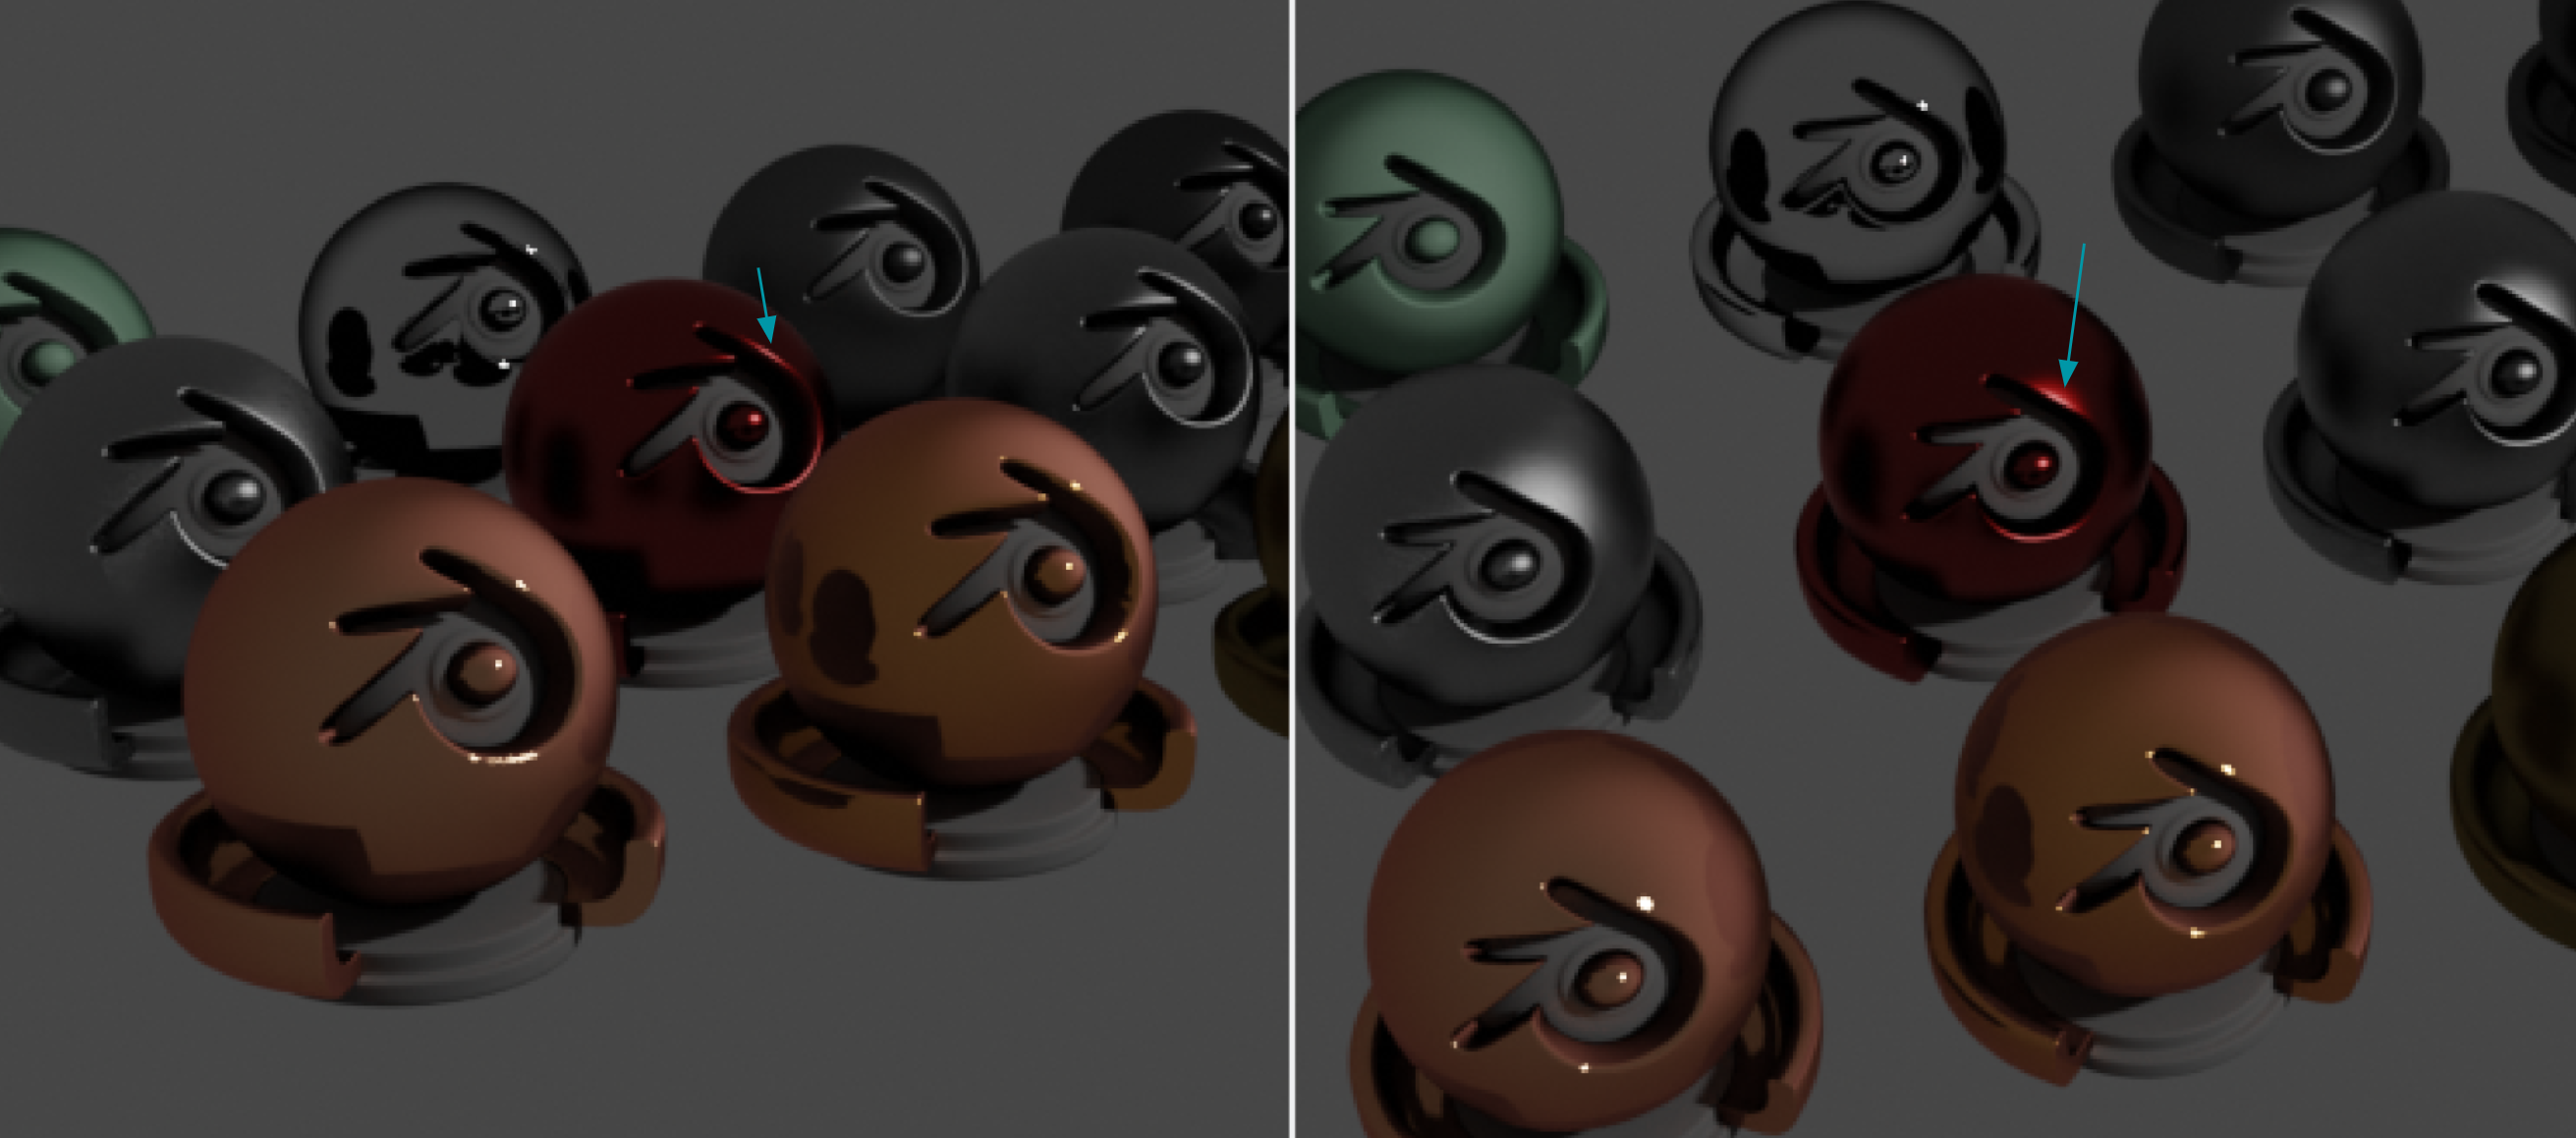
\includegraphics[width=0.4\textwidth]{figures/material_appearance_commented.png}
    \caption{Colors change with camera orientation, specular materials reflect the light and amplify this effect, the extreme use-case being mirrors.}
    \label{fig:material_changes}
\end{figure}

\noindent\textbf{Meshes.} Creating a mesh from the point cloud will lead to a nice geometric representation which can be rendered using classic rasterization techniques. But shading these triangles is still needed. If all materials are perfect diffusers, applying the textures extracted from the photos to the triangles shall be enough. Unfortunately, this will not work for specular materials as illustrated in figure \ref{fig:material_changes}. Neural deferred shading has been proposed \cite{worchel2022nds} to jointly fit a mesh while optimizing the pixel shader (mimicked by a neural network) of a classic mesh rendering pipeline (geometry processing $\rightarrow$ rasterization $\rightarrow$ \textit{(neural)} shader). Although mesh representations sounds flexible, the shading is baked into the scene representation and cannot be changed afterwards (for instance, lighting or materials cannot be changed).

\noindent\textbf{Neural radiance fields.} NERF \cite{mildenhall2020nerf} represents the scene RGB colors and density as a function of the 3D position and viewing angle. By shooting rays at the scene and sampling along them, one can integrate the estimated colors to render the final image\footnote{In this volumetric rendering, a density=0 means that the space is empty}. A MLP (Multi Layer Perceptron) is used to represent the radiance field. Having the dependance on the viewing angles allows to model complex materials and lighting effects. Main drawback is that NERF are computationally expensive as they require evaluating a MLP all along the rays for each pixel...

% A MLP can approximate basically any function as long as it has enough neurons...
\noindent\textbf{Point clouds.} Although point clouds are not continuous, they are a versatile representation of the scene and kind of easy to manipulate. The introduction of an additional inpainting method (e.g. neural rendering component) in the image space allows to overcome the limitations of the sparseness (see ~\cref{sec:methodology_paper}) while being able to render fast.

\subsection{Fast point based Rendering}
\label{subsec:Point based Rendering}
One of the major advantage of point based methods is that this technology is backed by years of prior industy work. Rendering point clouds can be hardware accelerated and is available to the mainstream public on basically any computer (without NVidia GPU). Libraries such as OpenGL offer the option to render points \texttt{GL\_Points} (and even specify the size of the splat \texttt{glPointSize(1);})... Point clouds can even be rendered in a web browser as shown in figure \ref{fig:potree}.

% https://github.com/rougier/python-opengl/blob/master/07-points.rst
% https://glumpy.github.io/

\begin{figure}[htbp]
    \centering
    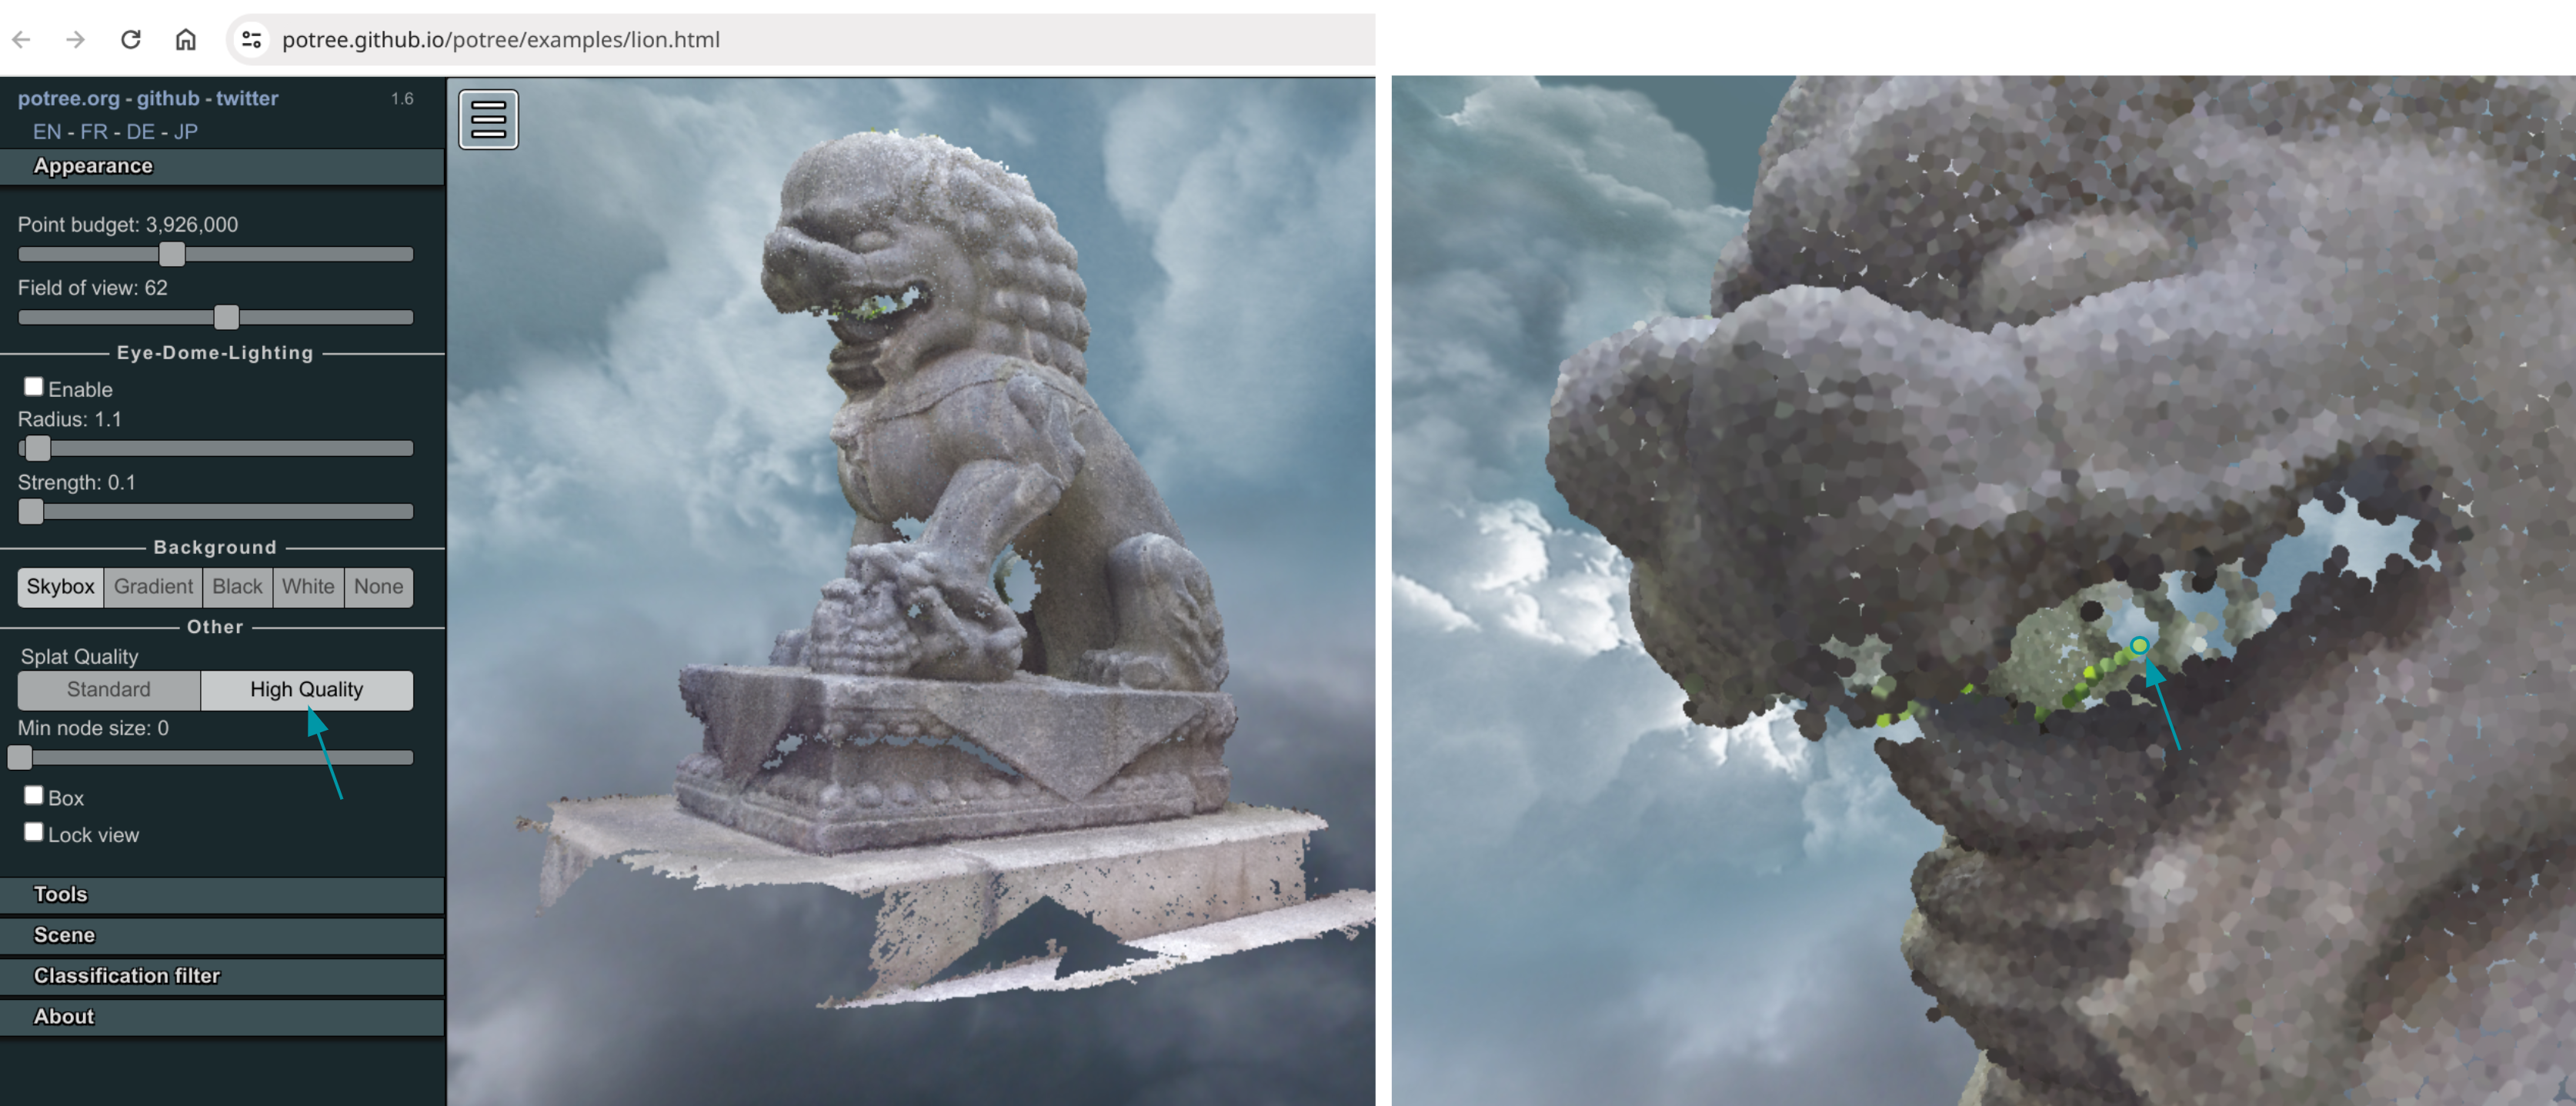
\includegraphics[width=0.45\textwidth]{figures/potree_rendering_and_splat.png}
    \caption{Potree \cite{potree} allows point cloud rendering in the browser, points being rendered as tiny circles splatted on the screen.}
    \label{fig:potree}
\end{figure}

\section{Original Paper overview}
\label{sec:methodology_paper}

NPBG \cite{Aliev2020} (Neural Point-Based Graphics) is a novel view synthesis method based on point cloud representation and introduced several important concepts (1. and 3. below).
ADOP \cite{Aruckert2022adop} adds a few components  (2. and 4.). to adapt to real scenes with high dynamic ranges and model complex camera pipelines.

\noindent\textbf{1. Geometry.} Learnable Pseudo-colors  \footnote{Pseudo-colors means a generic "feature" vector representation which can be more generic than three dimensional RGB components. A dimension 4 for instance.} assigned to each point are projected onto the camera screen at several scales. 

\noindent\textbf{2. Environment map.} A learnable 360° image is used to model the scene background.

\noindent\textbf{3. Neural rendering.} The multi-scale pyramid of pseudo images will be jointly decoded and inpainted into a RGB HDR \footnote{We define HDR as high dynamic range linear RGB images - as if they'd been retrieve from a RAW 12 or 14bit sensor with sole operations black point correction, demosaicing and potentially while balance/color matrix transforms.} image at full resolution, using a U-Net architecture.

\noindent\textbf{4. Camera simulation.} A camera simulation module will transform the image into a RGB LDR image \footnote{LDR stands for low dynamic range images, the ones we see on our screens after tone mapping, color adjustments like vibrancy, vigetting correction etc...}. 

\noindent An overview of the pipeline is shown in ~\cref{fig:original_pipeline}.
% TODO: ENVIRONMENT MAP!!!!!!!!!!!!!!!!!!!!!!!!!!!!!!!!!!!!!!!!!!!!!
\noindent The whole rendering pipeline is differentiable with regard to:
\begin{itemize}
    \item the pseudo-color of each point
    \item the environment map colors.
    \item the photometry camera parameters (exposure, white balance correction, tone curve parametric vignetting...)
    \item the camera pose and intrinsics \textit{This is an approximation, but it may be useful in order to refine camera pose estimation}. 
\end{itemize}

\noindent \textbf{Optimization} Using several photos of the scene for supervision, all parameters (network weights, pseudo-colors, environment map and camera photo pipeline) are optimized to minimize a loss function (MSE $\mathcal{L}^{2}$ or perceptual loss\footnote{Perceptual loss \cite{johnson2016perceptual} optimizes the distance between two images in a latent space rather than in the RGB colors space. We usually minimize the $\mathcal{L}^{2}$ distance between the feature maps in the middle of a frozen VGG network}) between predicted LDR rendered images and the real ones. 

\noindent\textbf{Implementation.} The authors wrote a C++ library (hybrid compiled code: lib Torch with cuda kernels and fast point rendering OpenGL code) to get fast trainings and reach impressive inference speeds: on scenes from Tanks and Temples \cite{Knapitsch2017TanksAndTemples} with 10 millions of points, they render the scenes at 37fps on a RTX3080 - 6 times faster than a NERF based method.

More details and limitations will be provided in the next sections.
